% ==================================================================================================================================
% Théorie des Langages

% - - - - - - - - - - - - - - - - - - - - - - - - - 
%                       TITLE
% - - - - - - - - - - - - - - - - - - - - - - - - - 


% - - - - - - - - - - - - - - - - - - - - - - - - - 
%               Chapters Inclusion
% - - - - - - - - - - - - - - - - - - - - - - - - - 

\chapter{Théorie des Graphes}

\minitoc 

% ==================================================================================================================================
% Introduction

\emph{Fiche réalisée grâce au cours de Thierry Montaut et Laura Brillon.}

Dans ce cours, on note $G = (X,E)$ un graphe.

% ==================================================================================================================================
% Graphes, Représentations et Parcours

\section{Graphes, Représentations et Parcours}

\subsection{Définitions - Graphes Orientés et Non Orientés}

\subsubsection{Vocabulaire}

\begin{definition}[Graphe non orienté]
    On appelle graphe non orienté un couple d'ensembles finis $G = (X,E)$ où $X = \{1, \dots, n\}$ représente les sommets du graphe
    et $E = \{ (x_i, y_j), \dots \}, x_i, y_j \in X$ l'ensemble des arrêtes du graphe. Une arrête est une liaison entre deux sommets.

    Un graphe est dit \textbf{simple} s'il n'existe pas de double arrêtes entre deux sommets ou de bouble (i.e une arrête de la forme $(x,x)$).
    Autrement, on parle de \textbf{multigraphe.}
\end{definition}

\begin{definition}[Graphe Orienté]
    On appelle graphe orienté un couple d'ensembles finis $G = (X,E)$ où $X = \{1, \dots, n\}$ représente les sommets du graphe 
    et $E = \{ (x_i, y_j), \dots \}$, $ x_i, y_j \in X$ l'ensemble ordonné des arrêtes du graphe. 
    Pour un graphe orienté, les notions de graphe simple et multiraphe sont les même que pour le cas non orienté.
\end{definition}

\begin{example}[Graphes et leur représentation graphique]
    Soient $G_1$ et $G_2$ deux graphes, en voici une représentation :
    \begin{figure}[h]
        \centering
        \begin{minipage}{0.45\textwidth}  % Première image dans 45% de la largeur de la page
          \centering
          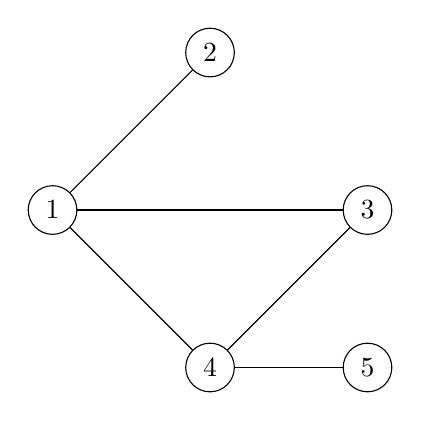
\begin{tikzpicture}[scale=1]
            % Déclaration des sommets avec des cercles
            \node[draw, circle] (1) at (0,0) {1};
            \node[draw, circle] (2) at (2,2) {2};
            \node[draw, circle] (3) at (4,0) {3};
            \node[draw, circle] (4) at (2,-2) {4};
            \node[draw, circle] (5) at (4,-2) {5};
      
            % Ajout des arêtes (non orientées)
            \draw (1) -- (2);
            \draw (1) -- (3);
            \draw (1) -- (4);
            \draw (4) -- (5);
            \draw (3) -- (4);
          \end{tikzpicture}
          \caption{Graphe non orienté}
          \label{fig:non-oriente}
        \end{minipage}%
        \hfill % Ajoute de l'espace flexible entre les deux images
        \begin{minipage}{0.45\textwidth}  % Deuxième image dans 45% de la largeur de la page
          \centering
          \begin{tikzpicture}[->,>=stealth',shorten >=1pt,auto,node distance=2cm,thick,scale=1]
            % Déclaration des sommets avec des cercles
            \node[draw, circle] (1) at (0,0) {1};
            \node[draw, circle] (2) at (2,2) {2};
            \node[draw, circle] (3) at (4,0) {3};
            \node[draw, circle] (4) at (2,-2) {4};
            \node[draw, circle] (5) at (4,-2) {5};
      
            % Ajout des arêtes orientées
            \draw[->] (1) -- (2);
            \draw[->] (1) -- (3);
            \draw[->] (4) -- (1);
            \draw[->] (2) -- (4);
            \draw[->] (3) -- (5);
          \end{tikzpicture}
          \caption{Graphe orienté}
          \label{fig:oriente}
        \end{minipage}
      \end{figure}
\end{example}

\begin{definition}[Planaire]
    Une graphe $G$ est dit planaire s'il existe une représentation de $G$ 
    en deux dimensions telle qu'aucun de ses sommets ne se croisent.
\end{definition}


\subsubsection{Voisinnage et degré}

\begin{definition}[Voisinnage]
    Le voisinnage d'un sommet $x$ de $G$ est l'ensemble des sommets $y$ de $G$ tels qu'il existe une arrête entre $x$ et $y$ dans $G$.
    On le note $V(x)$.
\end{definition}

\begin{remark}
    Si $x$ est dans le voisinnage de $y$, on dira que $x$ est adlascent à $y$ et inversement.
\end{remark}

\begin{definition}[Degré]
    Le degré d'un sommet $x$ de $G$ est le cardinal du voisinnage $x$. On le note $d(x)$.
    Un sommet de voisinnage nul est dit \textbf{isolé} et un sommet de voisinnage égal à 1 est dit \textbf{pendant}.
\end{definition}

\begin{definition}[Voisinnage entrant et sortant]
    Soit $G$ un graphe orienté et $x$ un sommet de $G$. On définit deux types de voisinnages :
    \begin{itemize}
        \item \textbf{Voisinnage entrant :} noté $V^-(X)$ est l'ensemble des prédécesseurs de $x$.
        \item \textbf{Voisinnage sortant :} noté $V^+(X)$ est l'ensemble des successeurs de $x$.
    \end{itemize}
    On définira comme précédemment le degré sortant et le degré entrant d'un sommet $x$.
\end{definition}


\subsubsection{Graphes Remarquables (non orientés)}

Dans cette sous-section, nous ne parlerons que de graphes non-orientés.

\begin{definition}[Graphe complet]
    On appelle graphe complet un graphe tel que pour tous sommets $x$ et $y$ de $G$ il existe une arrête entre $x$ et $y$ dans $G$.
    Les graphes complets $n$ sommets sont notés $K_n$
\end{definition}

\begin{remark}
    Autre définition de graphe complet et un petit peu d'histoire ne fera pas mal...
    \begin{itemize}
        \item On peut aussi définir un graphe complet comme étant un graphe dont tous ses sommets sont adjascents.
        \item  \emph{La notation $K$ pourrait avoir deux origines, la première étant en hommage à Kazimierz Kuratowski, 
        un éminent mathématiciens polonais ayant beaucoup contribué à la théorie des graphes. La seconde, plus simple, $K$
        proviendrait de sa traduction en Allemand komplett.}
    \end{itemize}
\end{remark}

\begin{example}
    Représentation des graphes complets $K_4$ et $K_5$ :
    \begin{figure}[h]
        \centering
        \begin{minipage}{0.45\textwidth}  % Première image dans 45% de la largeur de la page
            \centering
            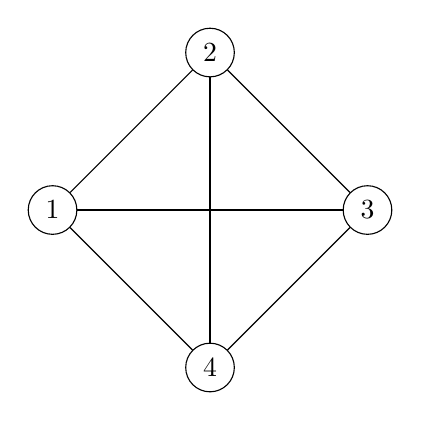
\begin{tikzpicture}[scale=1]
                % Déclaration des sommets avec des entiers pour K4
                \node[draw, circle] (1) at (0, 0) {1};
                \node[draw, circle] (2) at (2, 2) {2};
                \node[draw, circle] (3) at (4, 0) {3};
                \node[draw, circle] (4) at (2, -2) {4};
            
                % Ajout des arêtes pour K4 (chaque sommet est connecté aux autres)
                \draw (1) -- (2);
                \draw (1) -- (3);
                \draw (1) -- (4);
                \draw (2) -- (3);
                \draw (2) -- (4);
                \draw (3) -- (4);
              \end{tikzpicture}
              \caption{Graphe complet \( K_4 \)}
              \label{fig:K4-entiers}
        \end{minipage}
        \hfill % Ajoute de l'espace flexible entre les deux images
        \begin{minipage} {0.45\textwidth}  % Deuxième image dans 45% de la largeur de la page
            \centering
            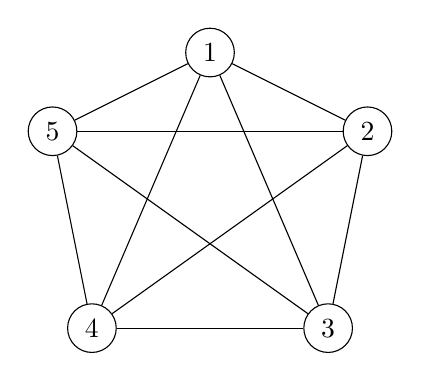
\begin{tikzpicture}[scale=1]
                % Déclaration des sommets avec des entiers pour K5
                \node[draw, circle] (1) at (0, 3.5) {1};
                \node[draw, circle] (2) at (2, 2.5) {2};
                \node[draw, circle] (3) at (1.5, 0) {3};
                \node[draw, circle] (4) at (-1.5, 0) {4};
                \node[draw, circle] (5) at (-2, 2.5) {5};

                % Ajout des arêtes pour K5 (chaque sommet est connecté aux autres)
                \draw (1) -- (2);
                \draw (1) -- (3);
                \draw (1) -- (4);
                \draw (1) -- (5);
                \draw (2) -- (3);
                \draw (2) -- (4);
                \draw (2) -- (5);
                \draw (3) -- (4);
                \draw (3) -- (5);
                \draw (4) -- (5);
            \end{tikzpicture}
            \caption{Graphe complet \( K_5 \)}
            \label{fig:K5-entiers}
        \end{minipage}
      \end{figure}
\end{example}

\begin{definition}[Bipartisme]
    Un graphe $G = (X,E)$ est dit biparti s'il existe une partition de $X$ en ensembles $X_1$ et $X_2$ non vides et disjoints tels que pour toute arrête $(x,y)$
    de $G$, $x$ et $y$ soient des ensembles différentes.
\end{definition}

\begin{remark}
    $G$ est dit $k$ parti, s'il existe une partition en $k$ ensembles de $X$ vérifiant la définition ci-dessus.
\end{remark}


\begin{example}
    Soit $G$ un graphe à 5 sommets biparti, alors :
    \begin{figure}[h]
        \centering
        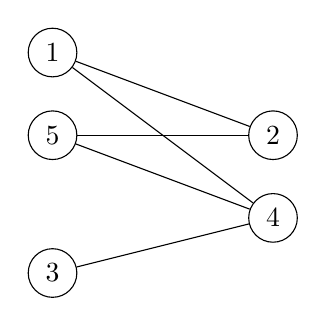
\begin{tikzpicture}[scale=0.7]
            \node[draw, circle] (1) at (-2, 4) {1};
            \node[draw, circle] (2) at (2, 2.5) {2};
            \node[draw, circle] (3) at (-2, 0) {3};
            \node[draw, circle] (4) at (2, 1) {4};
            \node[draw, circle] (5) at (-2, 2.5) {5};

            \draw (1) -- (2);
            \draw (1) -- (4);
            \draw (4) -- (3);
            \draw (4) -- (5);
            \draw (5) -- (2);
        \end{tikzpicture}
        \caption{Graphe biparti}
        \label{fig:K5-entiers}
    \end{figure}
\end{example}

\begin{example}[Graphe de Petersen]
    Sans doute l'un des graphes les plus connus en théorie des graphes, 
    le graphe de Pertersen en hommage à Julius Petersen qui l'étudia en 1898, possédant 10 sommets et 15 arrêtes possède 
    beaucoup de propriétés interressantes (notamment la connexité que nous verrons par la suite).
    Il est un contre-exemple pour beaucoup de propriétés et est très utile pour vérifier un algorithme en cours de développement ou une intuition. 
    \begin{figure}[h]
        \centering
        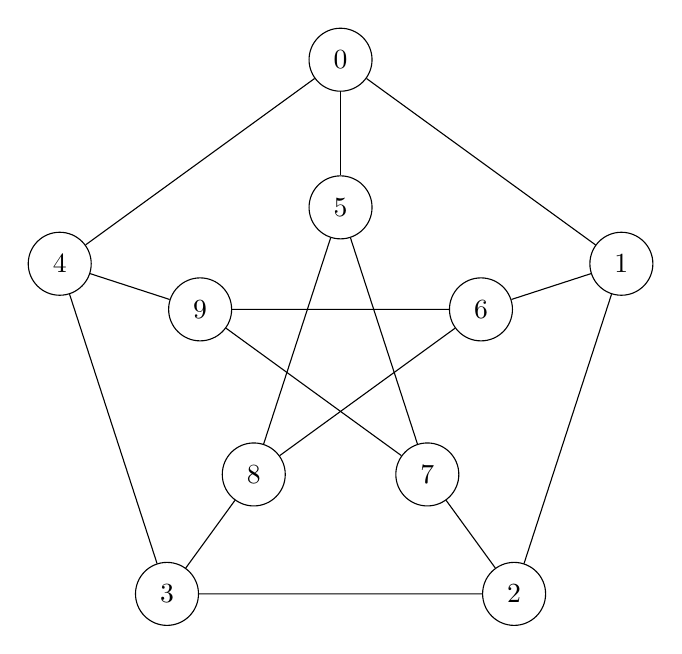
\begin{tikzpicture}[scale=1.25]

            % Coordonnées des sommets extérieurs
            \foreach \i in {0,1,2,3,4} {
                \node[circle, draw, minimum size=8mm] (a\i) at (90-\i*72:3) {\i};
            }
            
            % Coordonnées des sommets intérieurs
            \foreach \i in {5,6,7,8,9} {
                \node[circle, draw, minimum size=8mm] (b\i) at (90-\i*72:1.5) {\i};
            }
            
            % Arêtes du pentagone extérieur
            \foreach \i [count=\j from 1] in {0,1,2,3,4} {
                \pgfmathtruncatemacro{\nexti}{mod(\i+1,5)}
                \draw (a\i) -- (a\nexti);
            }
            
            % Arêtes du pentagone intérieur
            \foreach \i [count=\j from 1] in {5,6,7,8,9} {
                \pgfmathtruncatemacro{\nexti}{mod(\i+2,5)+5}
                \draw (b\i) -- (b\nexti);
            }
            
            % Arêtes reliant les sommets intérieurs aux sommets extérieurs
            \foreach \i in {0,1,2,3,4} {
                \pgfmathtruncatemacro{\j}{\i+5}
                \draw (a\i) -- (b\j);
            }
            
            \end{tikzpicture}
            \caption{Graphe de Petersen}
            \label{fig:K5-entiers}
    \end{figure}
\end{example}


\subsubsection{Propriétés}

\begin{prop}
    Soit $G$ un graphe non orienté simple à $n$ sommets.
    \begin{itemize}
        \item Si $G$ est complet, il possède $m =\frac{n(n-1)}{2}$ arrêtes.
        \item $G$ vérifie donc toujours $ m \leq \frac{1}{2} n (n-1)$
        \item $\sum_{x \in X} d(x)$ est le nombre d'extrémités d'arrêtes, c'est aussi deux fois le nombre d'arrêtes.
        \item Il y a un nombre pair de sommets de degré impairs.
    \end{itemize}
\end{prop}


\subsubsection{Graphes partiels et sous-graphes}

\begin{definition}[Graphe partiel]
    Soit $G = (X,E)$ un graphe. Le graphe partiel $G' = (X,E')$ de $G$ est tel que $E' \subset E$.
    Autrement dit, le graphe partiel d'un graphe $G$ est le même graphe mais avec quelques arrêtes en moins.
\end{definition}

\begin{definition}[Sous-graphe]
    Soit $G = (X,E)$ un graphe. Le graphe $G' = (X',E')$ de $G$ est tel que $X' \subset X$ et $E' = \{(x,y) : x \in X', y \in X', (x,y) \in E\}$.
    Autrement dit, le sous-graphe d'un graphe $G$ est le même graphe mais avec quelques sommets en moins (et donc quelques arrêtes en moins aussi).
\end{definition}

\begin{definition}[$k$-clique]
    Soit $G$ un graphe. On appelle $k$-clique, $k \leq n$, un sous-graphe complet de $G$de taille $k$.
\end{definition}


\subsubsection{Chaines et Cycles d'un graphe non orienté}

\begin{definition}[Chaine]
    On appelle chaine de $G$ de longueur $n$ toute suite alternée de sommets et d'arrêtes de $G$ telle que :
        \[ c = (x_0, a_1, x_1, \dots, a_n, x_n), \text{  telle que } \forall i \in \llbracket 1, n \rrbracket, a_i = (x_{i-1}, x_i) \]
    Ici, $n$ représente le nombre d'arrêtes de la chaine. Dans le cas d'un graphe simple, on notera les chaines de la façon suivante :
        \[ c = (x_0, \dots, x_n) \quad \text{ou} \quad c = x_0 - x_1 - \dots - x_n \] 
\end{definition}

\begin{definition}[Accessibilité]
    Soit $G = (X,E)$ un graphe. On a :
    \begin{itemize}
        \item Soient $x$ et $y$ deux sommets de $G$. On dit que $y$ est accessible à partir de $x$ s'il existe une chaine joignant $x$ et $y$ dans $G$.
        \item $G$ est dit \textbf{connexe} ssi $ \forall x \in X, \forall y \in X$, $y$ est accessible à partir de $x$.
        \item L'accessibilité est un relation d'équivalence entre les sommets. 
        
        Ses classes d'équivalences sont les composantes connexes de $G$.
    \end{itemize}
\end{definition}

\begin{definition}[Chaîne Simple]
    Une chaine est \textbf{simple} si elle ne passe pas deux fois par le même arrête et elle est dite élémentaire si elle ne passe pas deux fois pas le même sommet.
    On remarquera facilement qu'une chaîne élémentaire est simple.
\end{definition}

\begin{definition}[Cycle]
    Un cycle de $G$ est une chaine simple dont le départ et l'arrivée sont le même sommet. Un cycle est donc de la forme :
        \[ c = x_0 - x_1 - \dots - x_{n-1} - x0 \] 
\end{definition}

\begin{theorem}[Propriétés des cycles et chaînes]
    Soit $G$ un graphe.
    \begin{itemize}
        \item Toute chaine élémentaire a une longueur inférieure à $n-1$
        \item Toute cycle élémentaire a une longueur inférieure à $n$
        \item De toute chaîne, on peut en extraire une chaîne élémentaire.
    \end{itemize}
\end{theorem}


\subsubsection{Chemins, circuits d'un graphe orienté et forte connexité}

On utilise la même définition de chemin et circuit. Seulement, si le graphe est simple, il sera inutile de préciser les arrêtes par lesquelles on passe.

\begin{definition}[Forte Connexité]
    Un graphe $G = (X,E)$ orienté est dit fortement connexe si pour tout somet $x$ et $y$ de $G$, $y$ est accessible à partir de $x$.
\end{definition}


\begin{definition}[Arbre]
    On appelle arbre un graphe non orienté, connexe et sans cycle. Un graphe non orienté et sans cycle, i.e une union d'arbres et appelé \textbf{forêt}.
\end{definition}

\begin{theorem}[Caractérisation d'un arbre]
    Soit $T$ un graphe à $n$ sommets et $m$ arrêtes. $T$ est un arbre ssi :
    \begin{itemize}
        \item[\empty] $T$ est sans cycle et $m = n-1$ 
        \item[$\Longleftrightarrow$] $T$ est connexe et $m = n-1$
        \item[$\Longleftrightarrow$] $T$ est sans cycle et maximal au sens des arrêtes
        \item[$\Longleftrightarrow$] $T$ est connexe et minimal au sens des arrêtes 
        \item[$\Longleftrightarrow$] Deux sommets quelconques de $T$ sont reliés par un unique chemin.  
    \end{itemize}
\end{theorem}

% ==================================================================================================================================
% Représentation d'un graphe

\subsection{Représentations d'un graphe}

\subsubsection{Représentation par liste d'arrêtes}

\begin{definition}[Liste d'arrêtes]
    On appelle liste d'arrêtes de $G$ la liste des couples $(x,y)$ avec $x \in X$ et $y \in X$ tels que $(x,y) \in E$
\end{definition}


\begin{example} Représentations par liste d'arrêtes/d'arcs
    \begin{itemize}
        \item Le graphe orienté $G_1$ est représenté par la liste d'arcs :
            \[ [[1, 5], [2, 1], [2, 4], [3, 2], [4, 3], [5, 2], [5, 4]] \]
        \item Le multigraphe non orienté $G_2$ est représente par la liste d'arrêtes :
            \[  [[1, 2], [1, 5], [1, 5], [2, 1], [2, 4], [2, 4], [2, 3], [3, 2], [3, 3], [3, 4], [4, 2], [4, 2], [4, 3], [4, 5], [5, 1], [5, 1], [5, 4]] \] 
    \end{itemize}
    \begin{figure}[h]
        \centering
        \begin{minipage}{0.45\textwidth}  % Première image dans 45% de la largeur de la page
            \centering
            \begin{tikzpicture}[->,>=stealth',shorten >=1pt,auto,node distance=2cm,thick,scale=0.7]
                % Déclaration des sommets avec des entiers pour K4
                \node[draw, circle] (1) at (-1, 2) {1};
                \node[draw, circle] (2) at (1, 2) {2};
                \node[draw, circle] (3) at (2.5, 1) {3};
                \node[draw, circle] (4) at (1, 0) {4};
                \node[draw, circle] (5) at (-1, 0) {5};
            
                % Ajout des arêtes pour K4 (chaque sommet est connecté aux autres)
                \draw[->] (2) -- (1);
                \draw[->] (1) -- (5);
                \draw[->] (5) -- (4);
                \draw[->] (5) -- (2);
                \draw[->] (2) -- (4);
                \draw[->] (4) -- (3);
                \draw[->] (3) -- (2);
              \end{tikzpicture}
              \caption{Graphe Orienté $G_1$}
              \label{fig:K4-entiers}
        \end{minipage}
        \hfill % Ajoute de l'espace flexible entre les deux images
        \begin{minipage} {0.45\textwidth}  % Deuxième image dans 45% de la largeur de la page
            \centering
            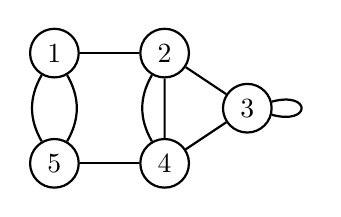
\begin{tikzpicture}[thick, scale=0.7]
                % Déclaration des sommets avec des entiers pour K5
                \node[draw, circle] (1) at (-1, 2) {1};
                \node[draw, circle] (2) at (1, 2) {2};
                \node[draw, circle] (3) at (2.5, 1) {3};
                \node[draw, circle] (4) at (1, 0) {4};
                \node[draw, circle] (5) at (-1, 0) {5};

                % Ajout des arêtes pour K5 (chaque sommet est connecté aux autres)
                \draw[bend left] (1) to (5);
                \draw[bend left] (5) to (1);
                \draw (5) -- (4);
                \draw (1) -- (2);
                \draw[bend right] (2) to (4);
                \draw (4) -- (2);
                \draw (4) -- (3);
                \draw (3) -- (2);
                \draw[loop right, -] (3) to ();
            \end{tikzpicture}
            \caption{Multigraphe non orienté $G_2$}
            \label{fig:K5-entiers}
        \end{minipage}
      \end{figure}
\end{example}

\subsubsection{Représentation Matricielle}

\begin{definition}[Matrice d'adjascence]
    On appelle matrice d'adjascence d'un graphe $G$ la matrice $A = (a_{ij})$ telle que 
    $\forall (i,j) \in X \times X$, on ait :
    \begin{itemize}
        \item Si $G$ est non orienté, $a_{ij}$ est égal à $1$ si $(i,j) \in E$ et $0$ sinon. La mrtice est donc symétrique.
        \item Si $G$ est orienté, $a_{ij}$ est égal à $1$ si $(i,j) \in E$
        \item Dans le cas d'un multigraphe, le coefficient $a_{ij}$ de la matrice d'adjascence de $G$ représente le nombre d'arrêtes entre les sommets $i$ et $j$ de $G$.
                Les coefficients diagonaux de la matrice représentent donc les boucles de $G$.
    \end{itemize}
\end{definition}


\begin{prop}
    Soit $G$ un graphe non orienté, et $A$ sa matrice d'adjascence.
    \begin{itemize}
        \item Puisque $G$ est non orienté, alors $A \in \mathcal{S}_n(\N)$ i.e $A$ est symétrique.
        \item La somme des éléments de la ligne $i$ est dégale à $d^-(i)$
        \item La somme des éléments de la colonne $i$ esy égale à $d^+(i)$
    \end{itemize}
\end{prop}

\begin{example}[Matrices d'adjascences]
    \begin{multicols}{2}
        La matrice d'adjascence de $G_1$ :
        \[ M_1 = 
        \begin{pmatrix}
            0 & 0 & 0 & 0 & 1 \\
            1 & 0 & 0 & 1 & 0 \\
            0 & 1 & 0 & 0 & 0 \\
            0 & 0 & 1 & 0 & 0 \\
            0 & 1 & 0 & 1 & 0 
        \end{pmatrix} \] 
        \vfill % Remplit l'espace verticalement pour ajuster la hauteur
        \columnbreak % Barre de séparation entre des deux colonnes
        La matrice d'adjascence de $G_2$ :
        \[ M_2 = 
        \begin{pmatrix}
            0 & 1 & 0 & 0 & 2 \\
            1 & 0 & 1 & 2 & 0 \\
            0 & 1 & 1 & 1 & 0 \\
            0 & 2 & 1 & 1 & 1 \\
            2 & 0 & 0 & 1 & 0
        \end{pmatrix} \] 
    \end{multicols}
\end{example}

\begin{remark}[Algèbre Linéaire]
    Comme dans toutes les représentations matricielles de concepts (que ce soit des applications ou des graphes),
    elles nous permettent d'invoquer facilement tous les résultats d'algèbre linéaires tels que la réduction,
    les noyaux, rangs, la composition...tout en préservant les propriétés des objets étudiés.
\end{remark}

\begin{prop}
    Soit $A^k, k \in \N$ où $A$ est la matrice d'adjascence d'un graphe $G$.
    Alors le coefficient d'indice $(x,y)$ de $A^k$ est le nomdre de chemins de longueur $k$ entre les sommets $x$ et $y$.
\end{prop}

\begin{remark}
    Toutefois, la représentation matricielle d'un graphe n'est pas optimale pour parcourir ces derniers puisque, ainsi, 
    les algorithmes de parcours auront forcément une complexité temporielle/spatiale en $\Theta(n^2)$.
\end{remark}

\subsubsection{Représentation par liste d'adjascence}

\begin{definition}[Liste d'adjascence]
    La liste d'adjascence d'un graphe $G$ est un vecteur $L$ indexé par $X$ tel que pour tout sommet $x \in X$,
    $L[x]$ est la liste des successeurs de $x$ dans $G$.
\end{definition}

\begin{example}
    Reprenons les graphes $G_1$ et $G_2$ représentés plus haut. On a alors :
    \begin{itemize}
        \item $G_1 = \{1 : [5],2 : [1,4],3 : [2],4 : [3],5 : [2,4]\}$
        \item $ G_1 = \{1 : [2,5,5],2 : [1,3,4,4],3 : [2,3,4],4 : [2,2,3,5],5 : [1,1,4]\}$
    \end{itemize}
\end{example}

\begin{remark}
    On remarque vite que cette représentation sera plus optinale. Premièrement, le parcours d'un graphe se fera en $\Theta(n)$ 
    et pour chaque sommet, on obtiendra sa liste de successeurs en $\Theta(1)$, si on représente une liste d'adjascence sous forme de dictionnaire en Python.
\end{remark}

\begin{prop}
    Pour chaque graphe à $n$ sommets et $m$ arcs, l'espace mémoire utilisé est un $\Theta(n+m) = \Theta (\max \{n,m\})$.
\end{prop}


\subsection{Parcours d'un graphe}

\subsubsection{Parcours en profondeur (Depth First Search)}

Le parcours en profondeur est à voir comme le parcours d'un chien fou dans un labyrinthe.
Celui-ci va partir dans un couloir et à chaque intersection va aller sur le chemin le plus proche jusqu'à arriver à une impasse.
A chaque impasse, il va revenir sur ses pas pour parcourir les autre chemins les plus proches. Le tout jusqu'à parcourir tout le labyrinthe.

Ainsi, cet algorithme de parcours se concevra de manière récurisive où chaque appel récurisif représentera l'envoi du chien fou dans un chemin (ici une arrête).
D'où l'algorithme suivant :

\lstset{
    basicstyle=\ttfamily\small,
    commentstyle=\color{green},
    keywordstyle=\color{blue},
    numbers=left,
    stepnumber=1,
    frame=single,
    breaklines=true
}
\begin{lstlisting}
Visite est initialise a l'ensemble vide 
Profond (G,x) :
    x est visite
    {Traiter x en premiere visite}
    Pour chaque voisin y de x faire :
        Si y n'est pas visite, alors :
            Profond(G,y)
        {Sinon on detecte une revisite de y}
    {Traiter x en derniere visite}
\end{lstlisting}


A partir du parcours en profondeur, on peut définir un ordre de parcours qui sera représenté par une liste de sommets.
Nous avons donc l'ordre de parcours en première visite (que l'on mettra à jour ligne 3 de l'algorithme)
et l'ordre de parcours en derniere visite (mis à jour ligne 9).

Pour un graphe $G$ non connexe ou non fortement connexe, le parcours en profondeur lancé à partir d'un unique sommet ne 
permettra pas d'accéder à tous ses sommets. D'où le parcours dit généralisé où l'on itère sur tous les sommets de $G$ et s'il n'est 
pas visité, on lance un parcours en profondeur à partir de celui-ci.

Ainsi, le parcours en profondeur généralisé d'un graphe $G$ permet de définir une arborescence de parcours.

\begin{definition}[Arborescence de parcours - profondeur]
    L'arborescence de parcours en profondeur de $G$ à partir d'un sommet $x \in X$ est une arbre $A$ enraciné en $x$, orienté, tel qu'il existe un arc $(x,y)$ dans $A$ 
    ssi l'appel à profond(G,x) a engendré récurisivement un appel à profond(G,y).
\end{definition}

A la fin d'un parcours en profondeur généralisé d'un graphe $G$, on obtient donc une forêt de visite contenant tous les sommets de $G$, i.e tous les sommets de $G$ ont étés visités.

\subsubsection{Parcours en largeur (Breadth First Search)}

Le parcours en largeur est fondamentalement différent de celui en profondeur. 
Tout d'abord, nous pouvons reprendre la comparaison avec le parcours d'un labyrinthe par un chien. 
Ici, notre chien sera vieux et plus malin. Pour chaque intersection (sommet), il va se rappeler de tous les chemins
à proximité (sommets voisins). Il se dirigera donc vers l'intersection (sommet) la plus ancienne qu'il ait retenue pour ensuite lister toutes
ses voisinnes, et ainsi de suite.
Pour ne pas tourner en rond, à chaque fois qu'il voit une intersection (sommet) voisinne, il vérifie qu'il ne l'aie pas visitée avant de la retenir.
Le vieux chien d'arrête donc dès qu'il n'a plus d'intersection (sommet) à visiter en mémoire.

On peut donc implémenter cette algorithme de façons itérative où un ensemble représentera les sommets déjà visités
et une file d'attente les sommets à visiter. Le premier sommet de file sera donc le prochain sommet à visiter.

\begin{lstlisting}
Visite est initilise a l'ensemble vide 
Largeur(G,x):
    F = [X]
    Visite[x] = vrai 
    Tant que F n'est pas vide, faire :
        Considerer la tete y de F et l'enlever de F 
        {Traiter y}
        Pour chaque successeur z de y, faire :
            Si z n'est pas visite, alors 
                z est visite 
                ajouter z a la fin de la file F 
\end{lstlisting}

De même que le parcours en profondeur, on peut définir un ordre de parcours, en première ou derniere visite.
Comme le parcours en profondeur, parfois nous auront besoin de lancer un parcours généralisé à tout le graphe pour parcourir tous ses sommets.

\begin{definition}[Arborescence de parcours - largeur]
    L’arborescence de parcours en largeur de $G$ à partir du sommet x est un arbre $A$  enraciné en x, orienté 
    tel qu’il existe un arc $(y,z)$ dans $A$ ssi le traitement de $y$ ajoute le sommet $z$ dans la liste d’attente $F$.
\end{definition}

La tableau Visite est intilisé en $\Theta(n)$. Le parcours est appelé exactement une seule fois pour chaque sommet $x$ de $G$ 
et a pour complexité $\Theta(1)$ pour le traitement de $x$ et $\Theta(d(x))$ pour l'exploration des successeurs de $x$.
La complexité des deux parcours est donc : 
\begin{align*}
    C(n) &= \Theta(n) + \sum_{x=1}^{n} (d(x) + \Theta(1)) \\ 
            &= \Theta(N) +  \sum_{x=1}^{n} d(x) \\
            &= \Theta(n) + \Theta(m) \\
            &= \Theta (\max \{n,m\})
\end{align*}


Maintenant que l'on sait parcourir un graphe, on peut étudier ses propriétés plus facilement.
Voici quelques exemples d'applications interressantes :

\subsubsection{Classification des arcs}

Une fois le parcours réalisé, on remarque que la forêt de parcours est composée de différents types d'arcs.
Soit $(x,y)$ un arc de $G$, il est dit...
\begin{itemize}
    \item \textbf{Couvrant} ssi $(x,y)$ est un arbre de la forêt de visite.
    \item \textbf{En avant} ssi il existe un chemin de $x$ à $y$ dans la forêt de visite de $G$.
    \item \textbf{En arrière} ssi il est chemin de $y$ à $x$ dans la forêt de visite.
    \item \textbf{Transverse} ssi ce n'est pas un arc ci-dessus.
\end{itemize}
La présence de cycle dans un graphe se manifestera par un arc arrière dans l'arbre de visite et un arc avant peut être vu comme un raccourci dans $G$.
Notons que pour chaque parcours, certains arcs sont présents et d'autres non.

\subsubsection{Existence de chemins et connexité}

Les deux parcours d'un graphe à partir d'un sommet $x$ nous permettent de trouver tous les sommets accessibles à partir de $x$.
Donc on peut facilement adapter un algorithme pour déterminer s'il existe un chemin entre deux sommets $x$ et $y$ de $G$, et même en trouver.

Dans le cas d'un graphe \textbf{non orienté}, si le parcours à partir d'un sommet $x$ atteint tous les autres sommets $y$ de $G$, alors $G$ est connexe et réciproquement.


\vspace{3cm}


\begin{quote}
    \centering
    \emph{"A partir d'ici, vous ne vous perdez plus dans les labyrinthes."} Thierry Montaut
    \justify
\end{quote}


% ==================================================================================================================================
% Modélisation et Graphes

\section{Modélisation et Graphes}

\subsection{Chemins et circuits Eulérien}

\subsubsection{Les 7 ponts de Königsberg}

Le problème des 7 ponts de Königsberg consiste à savoir s'il est possible de déterminer une promenade passant par tous les 
ponts de la ville de Königsberg en passant une et une seule fois par chaque ponts de la ville et en revenant à son point de départ. 
Ce problème est sûrement le plus connu de l'histoire de la théorie des graphes et fut résolut par \textbf{Leonhard Euler} en 1735. 
Il explique que le problème n'est pas résoluble pour la ville de Königsberg et établit ainsi l'un des tout premiers théorèmes 
de théorie des graphes. 

La démonstration mathématique du théorème d'Euler ne fut énoncée qu'en 1873 par Carl Hierholzer. 

Des problèmes similaires existent tels que celui du facteur chinois qui cherche à effectuer sa tournée de distribution en 
passant une et une seule fois par chaque rue et en revenant à son point de départ (Mai-Ko-Kwan, 1962).


\begin{definition}[Graphe Eulérien/Circuit Eulérien]
    Soit $G = (X,E)$ un graphe non orienté, un circuit eulérien dans $G$ est un circuit passant une et une seule 
    fois par chaque arrête et revenant au sommet de départ. 

    Un graphe est dit eulérien ssi il possède un circuit eulérien. 
\end{definition}

\subsubsection{Théorème d'Euler}

\begin{theorem}[Théorème d'Euler]
    Soit $G$ un graphe non orienté \textbf{connexe}. 
    \begin{itemize}
        \item $G$ admet un circuit eulérien ssi tous ses sommets sont de degré pair. 
        \item $G$ admet un circuit eulérien ssi tous ses sommets ont un degré pair seuf deux sommets $a$ et $b$
        alors, tous les circuits eulériens de $G$ on a/b comme sommet de départ et b/a comme sommet d'arrivée.  
    \end{itemize}
\end{theorem}

\subsubsection{Algorithme de recherche de circuits eulérien}

L'objectif de l'algorithme est de construire un circuit eulérien dans un graphe en considérant un graphe partiel
du graphe initial. A chaque étape, on cherche un chemin maximal partant du premier sommet non saturé du chemin précédent
et qui revient à ce sommet. Puisque il existe un nombre pair de sommets de degré impair il existe un tel sommet à chaque itération. 

A la fin de l'algorithme on "recolle" tous les chemins bout à bout en un seul chemin simple non extensible passant par toutes 
les arrêtes, créant ainsi un circuit eulérien. 

L'idée est de créer une "copie" du graphe et, lors de la création d'un chemin à une certaine étape, d'enlever les arrêtes concernées
par le chemin pour éviter qu'elles ne soient réutilisées. 


\subsection{Problème de coloration}

Les problèmes de colorations de graphes, en plus d'êtres difficiles à résoudre, sont, cependant, très facile à imaginer. 
L'exemple le plus typique est celui de la coloration d'une carte géographique. En essayant de colorier une carte de l'Europe
d'une telle façon que deux pays limitrophes n'aient pas la même couleur, on s'apperçoit vite que cela peut être compliqué, 
surtout si on essaye d'utiliser le moins de couleurs possibles.

C'est exactement ce que modélisent les problèmes de coloration de graphes. On essaye d'attribuer à chaque sommet une couleur
de telle sorte que tous ses voisins n'aient pas la même couleur que lui en utilisant le moins de couleurs possibles. 

\begin{definition}[$k$-coloration]
    Soit $G$ un graphe non orienté. On dit que $G$ admet une $k$-coloration s'il existe $k$ couleurs différentes 
    telles que deux sommets adjacents de $G$ n'aient pas la même couleur. 
\end{definition}

\begin{prop}[Propriétés des colorations]
    \begin{itemize}
        \item Si $G$ est $k$-parti alors $G$ est $k$-colorable. 
        \item Si $G$ est un graphe complet de taille $n$ alors $G$ ne peut pas être colorié avec moins de $n$ couleurs. 
        \item Si $G$ admet une $k$-clique, alors $G$ ne peut pas être colorié avec moins de $k$ couleurs.
    \end{itemize}
\end{prop}

\begin{definition}[Nombre Chromatique]
    On appelle nombre chromatique $\gamma(G) = k$ d'un graphe $G$ le plus petit entier positif tel que $G$ admette une $k$-coloration.
\end{definition}

\subsubsection{Coloration Naïve}

Premier algorithme de coloration de graphe, il est très facile à comprendre et à mettre en oeuvre mais 
est particulièrement gourmand en couleurs. 

L'idée est de parcourir le graphe dans l'ordre naturel des sommets et d'attribuer à chaque sommet 
la plus petite couleur non attribuée à ses voisins. 

Il faut donc une fonction permettant de parcourir le graphe et une autre déterminant 
la plus petite couleur non attribuée aux voisins d'un sommet. 
La coloration est représentée par un dictionnaire dont les clés sont les sommets 
du graphe et les valeurs, les couleurs attibuées aux sommets. 

C'est un algorithme très peut coûteux d'une complexité en $\Theta(m)$ mais pas très optimal, 
puisque en fonction de l'ordre de visite des sommets, le nombre de couleurs utilisées peut 
varier. Il est très peu efficace pour de gros graphes. 

\subsubsection{Coloration Gloutonne}

Prenez vos crayons de couleurs préférés et essayer de colorier un graphe. 
Vous alez d'abord colorier tous les sommets possibles avec un certaine couleurs. 
Puis une fois que vous ne pouvez plus colorier de sommets de cette couleur tel qu'aucun 
de ses voisins n'est déjà colorié vous prenez une autre couleur et refaites de même. 
Le tout jusqu'à ce que tous les commets soient coloriés. 

C'est le principe de l'algorithme de coloration Gloutonne. A chaque étape, on choisit une 
couleur et on essaye de colorier le maximum de sommets non adjacents avec cette même couleur. 
Pour cela, nous allons considérer le noyau d'une graphe. 

\begin{definition}[Noyau]
    Soit $G = (X,E)$ un graphe. On appelle noyau de G un ensemble maximal de sommets 
    non adjacents deux à deux. 
\end{definition}

On va donc déterminer tous les noyaux de G en détruisant petit à petit le graphe. 
Et, pour chaque noyau de trouvé, on colorie tous les sommets du noyau avec la même couleur. 


\subsection{Ordonnancement}

Ici, un graphe représente un système de dépendances entre différentes tâches d'un même projet. 
Chaque sommet repésente une tâche à effectuer et une arrête d'un sommet $x$ vers un sommet $y$ indique que 
la tâche $y$ doit attendre que la tâche $x$ est terminée avant d'être commencée. 

On va donc essayer d'établir un graphe d'ordonnancement des tâches visant à indiquer dans quel ordre les différentes 
tâche devront être traitées. Mais pour cela, il faut définir certaines conditions sur le graphe de dépendances. 

\begin{proposition}
    Soit $G = (X,E)$ un graphe. 
    \begin{itemize}
        \item Si G est sans circuit, alors tous ses sous-graphes sont sans circuits. 
        \item Si G est sans circuit, le graphe inverse de G est sans circuit. 
        \item G est sans circuit ssi tous ses chemins sont élémentaires. 
    \end{itemize}
\end{proposition}

\begin{definition}[Sommets remarquables d'un graphe sans circuit]
    Soit $G = (X,E)$ un graphe orienté sans circuit. On définit :
    \begin{itemize}
        \item une \textbf{source} comme étant un sommet dont le degré entrant est nul. 
        \item un \textbf{puit} comme étant un sommet dont le degré sortant est nul. 
    \end{itemize}
\end{definition}

\begin{theorem}[Fondamental de l'ordonnancement]
    Tou graphe sans circuit possède une source et un puit. 
\end{theorem}

\subsubsection{Tri Topologique - Ordonnancement séquentiel}

\begin{definition}[Tri Topologique]
    On appelle tri topologique d'un graphe orienté une numérotation des des sommets respectant l'ordre des arcs. 
\end{definition}

\begin{theorem}[Condition d'existence d'un tri topologique]
    Soit $G = (X,E)$ un graphe orienté. G admet un tri topologique ssi il est sans circuit. 
\end{theorem}

Le principe de l'algorithme de tri topologique est \textbf{itératif}. 
Il repose sur le fait que tout graphe sans circuit \textbf{possède une source}. 
On va donc, à chaque étape, chercher une source du graphe et l'insérer dans notre tri topologique. 
L'étape suivante, on \textbf{considère le sous-graphe} du graphe initial auquel on a enlevé la source et tous les 
arcs sortants. 

Si on ne souhaite pas détruire le graphe, on va considérer les \textbf{degrés entrants} de chaque sommets dans un \textbf{dictionnaire} des degrés.

\lstset{
    basicstyle=\ttfamily\small,
    commentstyle=\color{green},
    keywordstyle=\color{blue},
    numbers=left,
    stepnumber=1,
    frame=single,
    breaklines=true
}
\begin{lstlisting}
S:=[];T:=[];
Pour x de 1 a n faire
    Degre[x]:=d^-(x) dans G;
    Si Degre[x]=0 alors ajouter x a S;
{S contient alors toutes les sources de G}

Tant que S<>[] faire
    x:=enleverTete(S);
    ajouterFin(x,T)

    {Mettre a jour les degres}
    Pour chaque successeur y de x dans G faire
        Degre[y]:=Degre[y]-1;
        si Degre[y] = 0 alors ajouterFin(y,S)
\end{lstlisting}

L'algorithme repose donc sur un \textbf{parcours en largeur}. On utilise une \textbf{file} pour stocker les 
sommets de degré entrant nul (i.e les sources). A chaque itération, on décrémente tous les degrés entrants des fils de la source, 
puis on ajoute la source à la liste représentant le tri topologique. 


\subsubsection{Tri par Niveaux - Ordonnancement en parallèle}

Ici, comparé à un tri topologique, on va construire un graphe d'ordonnancement en considérant que l'on peut effectuer plusieurs 
tâches en même temps. 

\begin{definition}[Tri par niveaux]
    Soit $G = (X,E)$ un graphe orienté, sans circuit. 
    Un tri par niveaux de G est une partition de G en niveaux tels que pour chaque sommet d'un même niveaux, 
    son exécution n'est pas dépendante d'un sommet du même niveau ou d'un niveau suivant. 
\end{definition}

L'algorithme est sensiblement le même que le tri topologique. Il suffit juste de l'adapter 
pour \textbf{traiter en même temps} toutes les sources de G. 
On définit alors \textbf{deux listes N1 et N2} représentant deux niveaux successifs. 
Le traitement des sources de N1 permet de déterminer les sources de N2. 

\begin{lstlisting}
N1:=[];T:=[];
Pour x de 1 a n faire
    Degre[x]:=d^-(x) dans G;
    Si Degre[x]=0 alors ajouter x a N1;
{S contient alors toutes les sources de G}

tant que N1<>[] faire
    ajouterFin(N1,T);
    N2:=[];
    pour tout x dans N1 faire
        {Mettre a jour les degres des successeurs de x et calcul}
        Pour chaque successeur y de x dans G faire
        Degre[y]:=Degre[y]-1;
        si Degre[y] = 0 alors ajouterFin(y,N2)
    N1:=N2;
\end{lstlisting}


\subsection{Arbre couvrant de poids minimum}

Ici, on considère un \textbf{graphe non orienté valué }pour lequel on va chercher un sous-arbre couvrant de poids minimal. 
Cela peut éventuellement modéliser le problème d'un électricien qui doit relier différentes pièces par un câble 
et cherche à utiliser le moins de câble électrique possible. 

\begin{definition}[Valuation]
    Soit $G = (X,E)$ un graphe non orienté. Une valuation est une fonction 
    \[ p : E \longrightarrow \R \] 
    qui, à chaque arrête lui associe une valeur appelée poids. 

    Un graphe muni qu'un valuation est appelé graphe valué. 
\end{definition}

Pour \textbf{représenter} un graphe valué, nous allons toujours utiliser une liste d'adjacence. 
Mais nous allons rajouter une matrice de poids représentée par un dictionnaire dont les clés sont les arrêtes (couple)
et la valeur, le poids de l'arrête correspondante. 

On pourra aussi représenter un graphe valué par une liste d'arrêtes composée de triplet représentant les deux sommets de l'extrémité 
de l'arrête et le poids de l'arrête. 

\begin{definition}[Arbres couvrant]
    Soit $G = (X,E)$ un arbre graphe non orienté valué. 
    Un arbre couvrant de G est un graphe partiel de G, $A = (X,E')$ qui soit un arbre. 
\end{definition}

\begin{theorem}[Condition d'existence]
    Soit $G = (X,E)$ un graphe non orienté valué. G admet un arbre couvrant ssi il est connexe. 
\end{theorem}


\subsubsection{Algorithme de Kruskal}

L'algorithme de Kruskal construit de \textbf{manière itérative} un arbre couvrant de poids minimal. 
Pour cela, on va considérer les arrêtes par ordre de poids croissant. A chaque itération, on va essayer d'ajouter 
\textbf{la plus petite arrête ne créant pas de cycle} à l'arbre couvrant. 

On s'arrête lorsque l'on a ajouté $n-1$ arrêtes. 

\begin{remark} (Condition d'arrêt et vérification)
    \begin{itemize}
        \item A chaque itération, il faut vérifier que le graphe construit de possède pas de cycle, il faut donc effectuer 
            un \textbf{parcours en largeur}. 
        \item Si à une itération, on ne trouve pas d'arrête qui convienne, c'est que le graphe n'était initialement pas connexe. 
    \end{itemize}
\end{remark}

\subsubsection{Algorithme de Prim}

L'algorithme de Prim cherche, contrairement à Kruskal, à \textbf{conserver la connexité à moindre coût}. 

On va donc considérer deux ensembles :
\begin{itemize}
    \item C : l'ensemble des arrêtes de T (arbre couvrant)
    \item M : le complémentaire de C dans X 
\end{itemize}

A chaque étape, on va donc chercher une arrête \textbf{joignant un sommet de C à un sommet de M dans G. }
Un arrête joignant deux composantes connexe ne pouvant pas créer de cycle, le graphe T reste bien un arbre. 

On s'arrête lorsque \textbf{T contient tous les sommets de G}. 

% \subsubsection{Implémentation}

\begin{comment}
    \begin{lstlisting}
    {Initialisations}
    T:=[];m:=0;
    M:=[];
    connexe:=vrai
    Pour i de 1 à n faire
        DIST[i]:=p(x,i); {S’il n’y a pas d’arete (x,i) p(x,i) renv
        MIN[i]:=x
        Si i<>x alors ajouterfin(i,M)

    Tant que connexe et m<n-1 faire
        {(1) chercher l’arête (y,z) de poids minimal telle que y soit dans C et z dans M}
        z:=min(DIST); {pas la valeur mais l’indice}
        si z=0 {toutes les valeurs de DIST sont infinies} alors c
        Debut
        enlever(z,M);
        y:=MIN[z];
        u:=(yz);
        Ajouterfin(u,T);
        m:=m+1;
    \end{lstlisting}
\end{comment}


\subsection{Plus courts chemins dans un graphe valué}

On considère ici un \textbf{graphe orienté valué}. 
L'objectif est de trouver un chemins entre deux sommets $x$ et $y$ dans G de poids minimal. 
On retrouve le même problème pour le routage de paquets dans un réseau. En effet, lors de l'établissement 
des tables de routage, on va chercher le chemin le plus court (au sens de la durée de transfert) entre deux noeuds. 


\begin{definition}[Cycle Absorbant]
    Dans le cas d'un graphe orienté, valué à \textbf{poids négatifs}, on appelle cycle absorbant 
    un cycle de coût total négatif. 
\end{definition}

\begin{remark}
    Le passage par un cycle absorbant dans un tel graphe fait diminuer le coût du chemin de poids minimal. 
    On comprend alors vite qu'un graphe avec un circuit absorbant ne possède pas de chemin de poids minimal. 
\end{remark}

\begin{theorem}[Condition d'existence]
    Soit $G = (X,E)$ un grapge orienté valué. Soient $x$ et $y$ deux sommets de G. 
    Alors il existe un chemin de poids minimal entre $x$ et $y$ ssi 
    \begin{itemize}
        \item $y$ est accessible à partir de $x$ 
        \item G ne possède pas de circuit absorbant
    \end{itemize}
\end{theorem}


\subsubsection{Algorithme de Dijkstra}

L'algorithme de Dijkstra 1 se base sur un \textbf{parcours en largeur} du graphe. 
On cherche tous les plus courts chemins d'un sommet s vers les autres sommets du graphe. 
Pour cela on dispose d'un \textbf{dictionnaire des poids}, et d'un \textbf{dictionnaire des pères}. 


A l'initialisation, on commence par parcourir tous les sommets du graphe à la recherche d'arrêtes partant de s. 
On va construire pas à pas un plus court chemin vers chaque sommet. A chaque étape, on considère tous les "nouveaux"
chemins vers les sommets du voisinnage du sommet traité. Si on trouve un chemin plus court, on remplace le chemin actuel et on remet le sommet dans la file. 
Dans le cas contraire, on ne fait rien. 

\begin{lstlisting}
M:={s};
{Initialisation}
Pour i de 1 a n faire
    Si (s,i) est une arete alors
        D[i]:=cout(s,i);
        P[i]:=s;
        ajouter(i,M);
    Sinon D[i]:=infini;

{Algorithme}
Tant que M<>{} faire
    x:=enleveTete(M);
    Pour tout successeur y de x faire
        d:=D[x]+cout(x,y);
        si d<D[y] alors
            D[y]:=d;
            P[y]:=x;
            ajouter(y,M)
\end{lstlisting}

L'algorithme de Dijkstra possède quand même quelques inconvénients. 
Un même sommet peut se retrouver plusieurs fois dans la file et on visite donc tous ses voisins plusieurs fois. 
Dans le cas \textbf{d'arrêtes à poids tous positifs}, on peut éviter tous ces parcours inutiles choisissant à chaque étape le sommet
dont le chemin depuis s est de coût minimal.

\subsubsection{Dijkstra Opt}

A chaque fois que l'on récupérer un sommet dans la file, on va \textbf{récupérer le sommet de poids minimal.} 
Pour cela, on va \textbf{garder la file triée selon le poids des sommets}. Il faut donc implémenter un fonction 
\texttt{insere} qui ajoute un sommet dans la file en fonction de son degré d'accessibilité. 

\begin{lstlisting}
{Initialisations}
M:={};
Pour i de 1 a n faire
    Si (s,i) est une arete alors
        D[i]:=cout(s,i);
        P[i]:=s;    
        ajouter(i,M);
    Sinon D[i]:=infini;

{Algorithme}
Tant que M<>{} faire
    x:=choisir_min(M,d);
    enlever(x,M);
    Pour tout successeur y de x faire
        Si y est dans M alors
            d:=D[x]+cout(x,y);
            si d<D[y] alors
                D[y]:=d;
                P[y]:=x;
                ajouter(y,M)
\end{lstlisting}

La \textbf{complexité} de l'algorithme de Dijkstra est donc en $$ \boxed{ \Theta(n^2) + \Theta(m) = \Theta(n^2) }$$

\subsubsection{Algorithme de Floyd}

Cet algorithme permet de calculer \textbf{tous les plus courts chemins} de tous les sommets vers tous les autres. 
Il a un \textbf{complexité} en $\Theta(n^3)$, donc il reste très efficace. 

L'algorithme repose sur une \textbf{idée itérative}. On commence donc par calculer tous les plus courts chemins de i vers j (deux voisins)
sans intermédiaires. 
Puis on calcule tous les plus courts chemins avec \textbf{un intermédiaire.}
$$ \dots$$ 
Arrivé à la n-ième itération, on a tous les plus courts chemins du graphe. 

Par \textbf{récurence}, pour passer de l'étape k à l'étape k+1 :
    \[ \forall (i,j) \in \{1,n\}^2, \quad d = pcc[(i,k)] + pcc[(k,j)] \] 
    \[ \text{si } d < pcc[(i,j)]: \] 
    \[ \quad pcc[(i,j)] = d \] 

On utilise une \textbf{matrice de poids} (pcc) et un \textbf{dictionnaire des pères} P. 


\subsubsection{Algorithme de Bellman (poids quelconques)}

Ici, on cherche les plus courts chemins d'un graphe orienté valué avec potentiellement des poids négatifs. 

L'idée est que si on connaît tous les plus courts chemins d'un sommet s vers tous les prédécesseurs d'un sommet y de G, 
alors, le plus court chemin de s vers y est : 
    \[ min (\{d_i + p_i, \quad  i \in \{i,n\}\})=: d_{i0} + p{i0}\]
et le prédécesseur de y dans le plus court chemin sera $x_{i0}$. 

A \textbf{l'initialisation}, on connaît tous les plus courts chemins de $s$ vers lui-même. 
On considère donc $G'$ le \textbf{sous-graphe} de G constitué des sommets dont one ne connaît pas encore de plus courts chemins. 
$G'$ est un sous-graphe d'un graphe sans cycle donc il admet toujours des \textbf{sources}. 
Une source de $G'$ est un sommets de $G'$ dont on connaît tous les prédécesseurs. On peut donc calculer son plus courts 
chemin comme vu précédement et il sort de $G'$. 

On va construire un \textbf{dictionnaire des distances} \texttt{Dist} et un \textbf{dictionnaire des pères} dans le plus court chemin \texttt{Pred}. 
Pour l'algorithme, on utilise un dictionnaire représentant le nombre de prédécesseurs inconnus d'un sommet. 

\begin{lstlisting}
# Sort de G'
Pour x dans G[y] faire :
    Deg[x] -= 1
    si Deg[x] == 0 :
        ajouter(x,S)
\end{lstlisting}

\begin{lstlisting}
# calcul du pcc vers y
{Soit H la liste des predecesseurs dans G}
Pour x dans H[y] faire :
    si Dist[x] + P[(x,y)] < D[y] faire :
        D[y] = Dist[x] + P[(x,y)]
        Pred[y] = x 
\end{lstlisting}

Pour représenter le graphe on a donc besoin :
\begin{itemize}
    \item La liste d'adjacence de G.
    \item Le dictionnaire des pères.
    \item La matrice de poids représentée par un dictionnaire. 
\end{itemize}

L'algorithme se base donc sur un \textbf{parcours en  largeur}, d'où :

\begin{lstlisting}
{Initialisation}
...
{Algorithme}
Tant que S<>[] faire :
    y = tete de S 
    # calcul pcc vers y 
    # y sort de G'
\end{lstlisting}

Cet algorithme a donc un \textbf{complexité} en : 
    $$ \Theta(m + n) $$



\chapter{Mots et Langages}
\input{subjects/Graphes-Theorie-Langages/chapitres/chapitre1_Mots_Langages.tex}

\chapter{Automates (AFD, AFN, AF$\varepsilon$)}
\minitoc % Ajoute le sommaire local ici

% ==================================================================================================================================
% Introduction 

Comme abordé dans le chapitre précédent, on cherche une méthode pratique et efficace pour déterminer si un mot appartient 
à un langage ou pas. On veut donc un modèle qui soit d'une part très pratique mathématiquement pour nous permettre de 
démontrer des choses dessus mais aussi facilemet implémentable algorithmiquement. 

Alerte Spoiler : de solides connaissances en théorie des graphes seront plus qu'utiles...

% ==================================================================================================================================
% Automates fini déterministes

\section{Automates fini déterministes}

\subsection{Définition et représentation}

\begin{definition}[Automate fini déterministe]
    Un Automate Fini Déterministe est un quintuplet :
        \[ \boxed{ \mathcal{A} = (\Sigma, Q, T, q_0, A) } \] 
    où :
    \begin{itemize}
        \item $\Sigma$ est un alphabet 
        \item $Q$ est un ensemble fini d'états (souvent une partie finie de $\N$)
        \item $T : Q \times \Sigma \longrightarrow Q$ est une application qui, à un état et une lettre associe un autre état. 
        \item $q_0$ un état initial
        \item $A \subseteq Q$ les états acceptants
    \end{itemize}
\end{definition}

On représentera ainsi un automate fini déterministe de plusieurs façons en fonction de son utilisation :
\begin{itemize}
    \item \textbf{Mathématique : } $\mathcal{A} = (\Sigma, Q, T, q_0, A) $
    \item \textbf{Table de Transition : } Elle va permettre de trouver rapidement les différents types d'états. 
    \item \textbf{Sagitale : } Sous forme de graphe 
    \item \textbf{En Python : } Nous représenterons les automates finis déterministes sous la forme de quintuplet aussi. 
\end{itemize}

Regardons en détail ces différentes représentations au travers d'un exemple. 

\begin{example}
    Soit $\mathcal{A} = (\Sigma, Q, T, q_0, A)$ un automate fini déterministe. 

    \textbf{Mathématiquement} nous avons :
    \begin{itemize}
        \item $Q = \{1,2,3\}$ 
        \item $\Sigma = \{a,b\}$ 
        \item $q_0 = 1$ 
        \item $A = \{3\}$ 
    \end{itemize}
    
    La représentation \textbf{sagitale}  de notre automate sera :
        
        \begin{center}
            \begin{figure}[h]
                \centering
                \begin{tikzpicture}[shorten >=1pt, node distance=2cm, on grid, auto]
    
                    % Définitions des styles d'états
                    \node[state, initial] (1) {1};
                    \node[state, right=of 1] (2) {2};
                    \node[state, accepting, right=of 2] (3) {3};
                
                    % Définition des transitions
                    \path[->]
                    (1) edge[above] node{a} (2)
                    (2) edge[above] node{b} (3)
                    (2) edge[loop above] node{a} ()
                    (1) edge[loop above] node{b} ()
                    (3) edge[loop above] node{a} ()
                    (3) edge[loop below] node{b} ();
                
                \end{tikzpicture}
            \end{figure}
        \end{center}

    On représente de façon doublement cerclée les états acceptants. Les états sont les sommets du graphe. 
    Les arcs valués sont les antécédants/images de la fonction $T$. 

    Enfin, la \textbf{table de transition} de l'automate est représentée par le tableau suivant :
    \begin{multicols}{2}
        \begin{center}
            \begin{tabular}{c|c|c}
                Q/$\Sigma$ & a & b \\ \hline 
                1 & 2 & 3 \\ \hline 
                2 & 2 & 3 \\ \hline 
                \textbf{3} & 3 & 3 
            \end{tabular}
        \end{center}

        La première ligne présente les lettres de l'alphabet et la première colonne les différents états. 
        Pour chaque état, le tableau donne l'état obtenu en fonction de la lettre suivante lue. 
    \end{multicols}
\end{example}

\subsection{Mot et Langage Automatique}

\subsubsection{Lecture d'un mot}

\begin{definition}[Lecture d'un mot]
    Soit $\Sigma$ un dictionnaire, $l \in \Sigma$ et $\mathcal{A}$ un automate. 
    On lit la lettre $l$ en dérivant d'un état $q \in Q$ vers un état $q' \in Q$ et si $T(q,l) = q'$. 
    On notera la lecture d'un mot de longueur $p$ par la lecture successive de ses lettres :
        \[ q_1 \;  \overset{l_1}{\longrightarrow} \; q_2 \; \dots \; q_{p-1} \; \overset{l_p}{\longrightarrow} \; q_p \] 
\end{definition}

Concrètement, pour la lecture d'un mot, on va partir de l'état initial et en fonction des valeurs de l'état courant et de 
la lettre lue, on va "bouger" d'un état (sommet) à un autre.

\begin{definition}[Mot refusé]
    Un mot $w \in \Sigma^*$ est dit refusé par un automate $\mathcal{A}$ si sa lecture à partir de l'état initial 
    se termine sur un état refusant ou ne se termine pas. Dans le cas contraire, $w$ est dit accepté. 
\end{definition}

\begin{definition}[Langage d'un Automate]
    Le langage d'un automate $\mathcal{A}$ est l'ensemble des mots acceptés par l'automate. 
    On le note $L(\mathcal{A})$. 
\end{definition}

On parle de \textbf{langage automatique} si il est reconnaissable par un automate. 
Deux automates sont dits \textbf{équivalents} si ils reconnaissent le même langage. 

\subsubsection{Automate Complet}

\begin{definition}[Automate Complet]
    Un automate $\mathcal{A}$ est dit complet si 
        \[ \forall i \in Q, \forall l \in \Sigma, \quad T(i,l) \text{ est défini} \] 
    Autrement dit, un automate est dit complet si pour toute lettre et pour tout état fixés, il est possible de 
    changer d'état dans l'automate.  
\end{definition} 

\begin{definition}[Puit]
    Un état $q \in Q$ est un puit ssi 
        \[ \forall l \in \Sigma, \quad T(q,l) = q \]
    Un puit est un état duquel on ne peut sortir. 
\end{definition}

On définit aussi la notion de piège comme un puit refusant (i.e un puit dont l'état est refusant). 

\subsubsection{Complémentaire}

Puisque la notion de complémentaire existe pour les langages et que les automates semblent très étroitement liés 
aux langages, on peut se demander si un automate peut admettre un complémentaire... 

Soit $\mathcal{A}$ un automate associé à un langage L. On cherche $\mathcal{A}' = \overline{\mathcal{A}}$. 
    \[ w \in \overline{\mathcal{A}} \iff w \not \in L \iff w \not \in L(\mathcal{A}) \] 
Il semble falloir que $\mathcal{A}$ soit complet. Si c'est le cas, on pourrait inverser $\mathcal{A}$ en inversant 
les sommets accpetants/refusants. 

\begin{proposition}
    Tout automate fini peut être complété par des puits refusants en un automate complet. 
\end{proposition}

\begin{theorem}[Complémentarité]
    L'ensemble des automates est stable par complémentarité. 
\end{theorem}

% ==================================================================================================================================
% Automates fini non déterministes

\section{Automates fini non déterministes}

Dans la section précédente nous avons vu un modèle très efficace pour vérifier l'appartenance d'un mot à un langage. 
En plus d'être facilement représentable en mémoire (i.e Python), il est facile à utiliser à la main et 
hérite de toute la théorie des graphes vue précédement ce qui en fait un très beau modèle mathématiquement parlant. 

Malgré tout cela, nous ne savons pas comment, à partir de plusieurs langages simples, constituer un automate 
reconnaissant la somme de ces langages. Nous n'avons pas défini de somme/union d'automate et celles-ci semblent 
assez difficiles vu la rigidité de notre modèle. 

Nous allons donc construire un modèle d'automate, appelé non déterministe, nous permettant de faire ces opérations 
d'union (que nous appelerons juxtaposition). Elles nous permettrons de construire des automates complexes à partir de 
somme de langages. 


\subsection{Généralités}

\begin{definition}[AFN]
    Un automate fini non déterministe $ \mathcal{A}$ est un quintuplet : 
        \[ \mathcal{A} := (Q,\Sigma, T,I,A) \] 
    tel que :
    \begin{itemize}
        \item $Q$ est l'ensemble des états de l'automate 
        \item $\Sigma$ est un alphabet 
        \item $T : Q \times \Sigma \longrightarrow \mathcal{P}(Q)$ est une application 
        \item $I \subseteq Q$ est l'ensemble des états initiaux 
        \item $A \subseteq Q$ est l'ensemble des états acceptants. 
    \end{itemize}
\end{definition}

\begin{remark}
    Plusieurs remarques concernant ce nouveau modèle. Premièrement, on remarque que l'on peut maintenant définir 
    des transitions multiples entre les états de l'automate. Deuxièmement, il existe plusieurs états initiaux. 
\end{remark}

\subsubsection{Lecture d'un mot}

\begin{definition}[Arbre de lecture]
    Soient $w \in \Sigma^*$, $L$ un langage sur $\Sigma$ et $ \mathcal{A}$ un automate reconnaissant $L$.
    L'arbre de lecture de $w$ par $ \mathcal{A}$ est l'arbre résultat du parcours de $ \mathcal{A}$ en fonction 
    des lettres de $w$. 
    
    Autrement dit dans l'arbre de lecture G de $w$, un noeud $a$ est le fils d'un 
    noeud $b$ si il existe une lettre $l$ de $w$ telle que $T(b,l) = a$. Une feuille de cet arbre est un état acceptant 
    ou refusant de l'automate. 
\end{definition}

\begin{definition}[Lecture acceptante]
    Soient $w \in \Sigma^*$, $L$ un langage sur $\Sigma$ et $ \mathcal{A}$ un automate reconnaissant $L$. 
    Une lecture de $w$ par $ \mathcal{A}$ est dite acceptante si \underline{il existe} un chemin 
    d'un état initial vers un état acceptant dans l'arbre de lecture de $w$ par $ \mathcal{A}$. 
\end{definition}

\begin{proposition}
    On peut dire plusieurs choses de la lecture d'un mot $w \in \Sigma^*$ par un automate $ \mathcal{A}$ :
    \begin{itemize}
        \item Si l'automate possède plusieurs états initiaux, la lecture produit un arbre de lecture pour chaque 
        état initial, nous auront donc une \underline{forêt d'arbres de lecture}. 
        \item Une lecture sera donc acceptante ssi il existe un arbre de la forêt dont au moins une des feuilles
        est un état acceptant. 
    \end{itemize}
\end{proposition}

\begin{example}
    Voyons tout cela sur un exemple. Soit $ \mathcal{A} := (Q,\Sigma, T,I,A)$ un automate fini non déterministe $ \mathcal{A}$
    sur l'alphabet $\Sigma : \{a,b\}$. Représentons notre automate sous forme de graphe orienté valué et sa table de transition :
    \begin{center}
        \begin{minipage}{0.45\textwidth} % Colonne pour le dessin
            \begin{tikzpicture}[shorten >=1pt, node distance=3cm, on grid, auto]
    
                % Définitions des styles d'états
                \node[state, initial] (1) {1};
                \node[state, accepting, right=of 1] (2) {2};
                \node[state, below=of 1] (3) {3};
                \node[state, initial, right=of 3] (4) {4};
            
                % Définition des transitions
                \path[->]
                (1) edge[above] node{$a$} (2)
                (1) edge[left] node{$a$} (3)
                (2) edge[right] node{$a$} (4)
                (3) edge[below] node{$b$} (4)
                (4) edge[sloped, below left] node{$b$} (1)
                (4) edge[loop below] node{$b$} (4);
            
            \end{tikzpicture}
        \end{minipage}%
        \hfill 
        \begin{minipage}{0.45\textwidth} % Colonne pour le tableau
            \begin{tabular}{c|c|c}
                T & a & b \\ \hline 
                $1$ & $\{2,3\}$ & X \\ \hline 
                \textcircled{2} & $4$ & X \\ \hline 
                $3$ & X & $4$ \\ \hline 
                $4$ & X & $\{1,4\}$ 
            \end{tabular}
        \end{minipage}
    \end{center}
    C'est un automate non déterministe puisqu'il contient deux transitions mutliples et deux états initiaux. 

    Posons $w := abba$, déterminons si ce mot appartient au langage $L( \mathcal{A})$. Nous allons construire 
    un seul arbre permettant d'avoir une condition suffisante de validation du mot. 

    \begin{center}
        \begin{minipage}{0.45\textwidth}
            \begin{tikzpicture}[scale=0.8, transform shape, shorten >=1pt, node distance=3cm, on grid, auto]
                
                % Racine
                \node[state, initial] (1) {1};
    
                % 1er niveau
                \node[state] (2) [below right=2cm and 2cm of 1] {2};
                \node[state] (3) [below left=2cm and 2cm of 1] {3};
    
                % 2nd niveau
                \node[state] (x1) [below=2cm of 2] {X};
                \node[state] (4) [below=2cm of 3] {4};
                
                % 3eme niveau 
                \node[state] (42) [below left=2cm and 2cm of 4] {4};
                \node[state] (12) [below right=2cm and 2cm of 4] {1};
    
                % 4 eme niveau 
                \node[state] (22) [below right=2cm and 2cm of 12] {2};
                \node[state] (32) [below left=2cm and 2cm of 12] {3};
                \node[state] (x2) [below=2cm of 42] {X}; 
    
                % Branches
                \path[->]
                (1) edge[left] node{a} (2)
                (1) edge[left] node{a} (3)
                (2) edge[left] node{b} (x1)
                (3) edge[left] node{b} (4)
                (4) edge[left] node{b} (12)
                (4) edge[left] node{b} (42)
                (12) edge[left] node{a} (22)
                (12) edge[left] node{a} (32)
                (42) edge[left] node{a} (x2);
    
            \end{tikzpicture}
        \end{minipage}
        \hfill 
        \begin{minipage}{0.45\textwidth}
            L'arbre de lecture du mot $abba$ contient un état acceptant comme feuille. 

            \vspace{1cm}

            Autrement dit, il existe un chemin menant d'un état initial à un état acceptant dans la forêt de lecture 
            de $abba$. Donc $abba \in L( \mathcal{A})$. 
        \end{minipage}        
    \end{center}
\end{example}

\subsection{Juxtaposition et construction d'un AFD}

\subsubsection{Juxtaposition}

Rappelons la problématique principale du chapitre. On cherche un modèle dérivant des AFD nous permettant de définir 
des opérations dessus et qui puisse être convertit algorithmiquement vers un AFD pour construire des automates 
d'un langage complexe à partir de langages plus simple. 

Autrement dit, on veut pouvoir appliquer l'opération de somme de langages sur les automates fini déterministes. 

\begin{definition}[Juxtaposition d'AFN]
    Soient $L_1$ et $L_2$ deux langages reconnus par deux automates $ \mathcal{A}_1$ et $ \mathcal{A}_2$. 
    Le langage $L_1 + L_2$ est reconnu par la \textbf{juxtaposition disjointe} de $ \mathcal{A}_1$ et $ \mathcal{A}_2$. 
\end{definition}

\begin{theorem}[Langages automatiques et stabilité]
    L'ensemble des langages automatiques est stable par somme. 
\end{theorem}

On peut maintenant, à partir de deux langages automatiques, définir le nouveau langage résultant de 
la somme des deux qui sera lui aussi automatique. Il suffit de faire la juxtaposition disjointe des deux automates
de départ. 

\subsubsection{Déterminisation}

\begin{theorem}[Existence et équivalence]
    Pour tout automate fini non déterministe, il existe un automate déterministe équivalent. 
\end{theorem}

Ce théorème est peut être un peu obscur mais permet de dire qu'il est toujours possible de passer d'un 
automate fini non déterministe (obtenu par exemple par juxtaposition) à un automate fini déterministe
qui reconnaisse le même langage. En tout cas, il nous dit qu'il en existe un...


L'intérêt de vouloir repasser chez les automates fini déterministes vient du fait que la lecture d'un mot par 
un AFN est de complexité exponentielle alors que la lecture d'un mot par un AFD est polynômiale... 
Lors de la vérification syntaxique de très long mots pour des langages très complexes, cela fait une différence 
cruciale pour la compilation. 

Ce processus est appelé \textbf{déterminisation} d'un AFN. 

\begin{proposition}
    Soit $ \mathcal{A} = (Q, \Sigma, T, I, A)$ un AFN. On cherche à construire un AFD $ \mathcal{A}'$ équivalent à $ \mathcal{A}$. 
    L'idée est de raisonner sur l'application $T : Q \times \Sigma \longrightarrow \Q$. Dans un AFN, cette application 
    n'est pas injective, on va donc poser une nouvelle application dans l'espace quotient de $Q \times \Sigma$ par le noyau de $T$. 
    Nous obtiendrons donc une application injective et donc un AFD. 
\end{proposition}


\begin{example}[Déterminisation]
    Soit $ \mathcal{A}$ l'automate défini sur l'alphabet $\Sigma = \{ a,b \}$ non déterministe et sa table 
    de transition suivants : 

    \begin{center}
        \begin{minipage}{0.45\textwidth} % Colonne pour le dessin
            \begin{tikzpicture}[shorten >=1pt, node distance=3cm, on grid, auto]
    
                % Définitions des styles d'états
                \node[state, initial] (1) {1};
                \node[state, accepting, right=of 1] (2) {2};
                \node[state, initial, below=of 1] (3) {3};
                \node[state, right=of 3] (4) {4};
            
                % Définition des transitions
                \path[->]
                (1) edge[above] node{$a$} (2)
                (1) edge[left] node{$a$} (3)
                (2) edge[right] node{$a$} (4)
                (3) edge[below] node{$b$} (4)
                (4) edge[sloped, below left] node{$b$} (1)
                (4) edge[loop below] node{$b$} (4)
                (2) edge[loop above] node{$b$} (2)
                (3) edge[loop below] node{$a$} (3);
            
            \end{tikzpicture}
        \end{minipage}%
        \hfill 
        \begin{minipage}{0.45\textwidth} % Colonne pour le tableau
            \begin{tabular}{c|c|c}
                T & a & b \\ \hline 
                $1$ & $\{2,3\}$ & X \\ \hline 
                \textcircled{2} & $4$ & $2$ \\ \hline 
                $3$ & $3$ & $4$ \\ \hline 
                $4$ & X & $\{1,4\}$ 
            \end{tabular}
        \end{minipage}
    \end{center}

    Déterminisons cet automate. Pour cela, nous allons renommer tous les états de l'automate en prenant en 
    compte les ensembles. 
    L'algorithme consiste donc à construire la table de transition du nouvel automate. 
    Pour chaque itération (i.e ajout d'une ligne dans la table), on effectue un parcours en largeur du nouvel automate 
    pour "découvrir" de nouveau état. On créé ainsi un "automate des parties". 

    \begin{figure}[h]
    \begin{center}
        \begin{minipage}{0.45\textwidth}
            \begin{tabular}{c|c|c}
                & a & b \\ \hline 
                $I = \{1,3\}$ & $II$ & $III$ \\ 
                $II = \{2,3\}$ & $IV$ & $V$ \\ 
                $III = \{4\}$ & - & $VI$ \\ 
                $IV = \{3,4\}$ & $VII$ & $VI$ \\ 
                $V = \{2,4\}$ & $III$ & $ VIII$ \\ 
                $VI = \{1,4\}$ & $ II$ & $VI$ \\ 
                $VII = \{3\}$ & $VII$ & $III$ \\ 
                $VIII = \{1,2,4\}$ & $IX$ & $VIII$ \\ 
                $IX = \{2,3,4\}$ & $IV$ & $VIII$ 
            \end{tabular}
            \caption{Table de l'AFD}
        \end{minipage}
        \hfill 
        \begin{minipage}{0.45\textwidth}
            \begin{tikzpicture}[scale=0.8, transform shape, shorten >=1pt, node distance=3cm, on grid, auto]
                % 1er niveau
                \node[state] (I) {I};

                % 2nd niveau
                \node[state] (II) [below left=2cm and 2cm of I] {II};
                \node[state] (III) [below right=2cm and 2cm of I] {III};

                % 3eme niveau
                \node[state] (IV) [below left=2cm and 2cm of II] {IV};
                \node[state] (V) [below right=2cm and 2cm of II] {V};
                \node[state] (VI) [below=2cm of III] {VI};

                % 4eme niveau
                \node[state] (VII) [below=2cm of IV] {VII};
                \node[state] (VIII) [below=2cm of V] {VIII}; 

                % 5eme niveau
                \node[state] (IX) [below=2cm of VIII] {IX};
                
                % Branches 
                \path[-]
                (I) edge[left] node{a} (II)
                (I) edge[left] node{b} (III)
                (II) edge[left] node{a} (IV)
                (II) edge[left] node{b} (V)
                (III) edge[left] node{b} (VI)
                (IV) edge[left] node{} (VII)
                (V) edge[left] node{} (VIII)
                (VIII) edge[left] node{} (IX);
            \end{tikzpicture}
            \caption{Automate des parties}
        \end{minipage}
    \end{center} 
    \end{figure}
\end{example}

% ==================================================================================================================================
% Automates fini à espilon transitions

\section{Automates fini à $\varepsilon$-transitions}

Définissons un nouveau type d'automates non déterministes. Les automates non déterministes à $\varepsilon$-transition. 
Il diffèrent des premiers puisque l'on va permettre le changement d'état sans lecture de lettres lors 
de la lecture d'un mot. Pour cela, nous allons définir une transition $\varepsilon$. 
Cela peut se voir comme une transition via le mot vide. 

\subsection{Généralités}

\begin{definition}[Automate Fini à $\varepsilon$-transitions (AFN$\varepsilon$)]
    Un automate fini à $\varepsilon$-transitions est un quintuplet: 
        \[ \mathcal{A} = (Q,\Sigma, T, I, A) \] 
    définit de la même façon que les automates précédents mais où: 
        \[ T : Q \times \Sigma \cup \{\varepsilon\} \longrightarrow \mathcal{P}(Q) \] 
\end{definition}

Ici, le changement spontané d'état sans lecture de lettre sera donc caractérisé par une nouvelle 
entrée dans la table de transition $\varepsilon$. 

\begin{example}
    Soit le langage $L := a^*b^*$. Un automate reconnaissant ce langage peut être écrit avec une 
    $\varepsilon$-transition. Ecrivons aussi sa table de transition: 
    \begin{center}
        \begin{minipage}{0.45\textwidth} % Colonne pour le dessin
            \begin{tikzpicture}[shorten >=1pt, node distance=3cm, on grid, auto]
    
                % Définitions des styles d'états
                \node[state, initial] (1) {1};
                \node[state, accepting, right=of 1] (2) {2};
            
                % Définition des transitions
                \path[->]
                (1) edge[above] node{$\varepsilon$} (2)
                (1) edge[loop below] node{$a$} (1)
                (2) edge[loop below] node{$b$} (2); 

            \end{tikzpicture}
        \end{minipage}%
        \hfill 
        \begin{minipage}{0.45\textwidth} % Colonne pour le tableau
            \begin{tabular}{c|c|c|c}
                T & a & b & $\varepsilon$ \\ \hline 
                1 & 1 & - & 2 \\ \hline 
                \textcircled{2} & - & 2 & - \\ \hline 
            \end{tabular}
        \end{minipage}
    \end{center}
\end{example}

Lors de la lecture d'un mot, les transitions peuvent être très aléatoires en fonction du nombre 
d'$\varepsilon$-transitions possibles de l'état courant. Un tel automate est donc hautement non déterministe. 


\begin{definition}[Lecture d'un mot]
    Soit $w = l_1 l_2 \dots l_n $ un mot sur $\Sigma$. 
    Soit $w' = a_1 a_2 \dots a_p$ le mot $w$ $\varepsilon$-complété (rembourré par des $\varepsilon$) tel que :
    \begin{itemize}
        \item $p \geqslant n$ 
        \item $ \forall i \in \llbracket 1, n \rrbracket, \; a_i \in \{l_1, \dots, l_n\} \cup \{\varepsilon\}$ 
        \item $l_1 l_2 \dots l_n = a_1 a_2 \dots a_p$ (du point de vue du produit de concaténation)
    \end{itemize}
    Une lecture du mot $w$ par $ \mathcal{A}$ est une lecture par $ \mathcal{A}$ de n'importe quel $w'$, 
    un $\varepsilon$-complété de $w$. 
\end{definition}

\begin{remark}
    Tout comme pour les automates précédants, un mot appartient au langage d'un automate ssi 
    la lecture de ce mot par celui-ci se finit sur au moins un état acceptant de l'automate. 

    \vspace{0.3cm}

    La lecture d'un mot par un AFN$\varepsilon$ conduira donc à la construction d'une forêt de lecture de ce mot 
    par l'automate. 
\end{remark}

\begin{example}[Lecture d'un mot]
    Soit l'automate fini non déterministe à $\varepsilon$-transitions précédent. 
    Soit le mot $abb$. Construisons la forêt de lecture de $abb$ par $ \mathcal{A}$. 

    \begin{center}
        \begin{tikzpicture}[shorten >=1pt, node distance=3cm, on grid, auto, scale=0.7]
    
            % Définitions des styles d'états
            \node[state, initial] (1) {1};
            \node[state, accepting, below=of 1] (2) {2};
            \node[state, right=of 1] (11) {1};
            \node[state, right=of 2, xshift=-1.1cm] (X1) {X};
            \node[state, right=of 11] (X2) {X};
            \node[state, below=of 11] (22) {2};
            \node[state, right=of 22] (222) {2};
            \node[state, accepting, right=of 222] (2222) {2};
        
            % Définition des transitions
            \path[->]
            (1) edge[above] node{$a$} (11)
            (1) edge[right] node{$\varepsilon$} (2)
            (2) edge[above] node{} (X1)
            (11) edge[above] node{} (X2)
            (11) edge[right] node{$\varepsilon$} (22)
            (22) edge[above] node{$b$} (222)
            (222) edge[above] node{$b$} (2222);
    
        \end{tikzpicture}
    \end{center}

    Il existe un chemin d'un racine vers une feuille acceptante dans la forêt de lecture: 
        \[ 1 \overset{a}{\longrightarrow} 1 \overset{\varepsilon}{\longrightarrow} 2 \overset{b}{\longrightarrow} 2 \overset{b}{\longrightarrow} 2 \] 
    Donc par définition, $abb \in L( \mathcal{A} )$. 
\end{example}

\subsection{Déterministation}

Dans le chapitre précédent, un théorème nous permet de dire que pour tout automate fini non déterministe, 
il existe un automate fini déterministe équivalent. Ainsi, à chaque fois que l'on considère un AFN$\varepsilon$, 
on est sûr qu'il existe un AFD équivalent. 

Pour la déterminisation d'un AFN$\varepsilon$, nous allons avoir besoin d'une définition supplémentaire... 

\begin{definition}[Clôture]
    Soit $\mathcal{A} = (Q,\Sigma, T, I, A)$ un AFN$\varepsilon$. 
    Pour tout $q \in Q$, on appelle clôture de $q$ l'ensemble des états accessibles à partir de $q$ sans lecture de 
    lettre lors de la lecture d'un mot dans l'automate. 

    Autrement dit, la clôture de $q$ est l'ensemble des états accessibles depuis $q$ dans le sous-graphe de $ \mathcal{A}$
    restreint aux $\varepsilon$-transitions. 
    
    On note $cl(q)$ la clôture de $q$. 
\end{definition}


L'idée de la déterministation d'un AFN$\varepsilon$ est, non plus de regrouper des états, mais d'étendre les transitions 
de l'automate à tous les états accessibles par $\varepsilon$-transitions. 

De plus, si un état acceptant est accessible uniquement par $\varepsilon$-transtion depuis un état, alors celui-ci 
hérite du caractère acceptant de l'état atteint. 

\begin{proposition}[Algorithme de Déterministation]
    Soit $\mathcal{A} = (Q,\Sigma, T, I, A)$ un AFN$\varepsilon$. On construit l'automate fini déterministe $ \mathcal{A}'$ 
    équivalent à $ \mathcal{A}$ en :
    \begin{enumerate}
        \item Calculer les clôtures de $ \mathcal{A}$ 
        \item Héritage : Tous les états dont la clôture contient un état acceptant sont acceptants. 
        \item Calculer les transitions étendues 
        \item Déterminisation de $ \mathcal{A'}$ par l'automate des parties (voir chap précédent)
    \end{enumerate}
\end{proposition}

\begin{example}[Déterminisation]
    Soit $ \mathcal{A}$ l'AFN$\varepsilon$ suivant : 
    
    \begin{center}
        \begin{minipage}{0.7\textwidth} % Colonne pour le dessin
            \begin{tikzpicture}[shorten >=1pt, node distance=3cm, on grid, auto]
    
                % Définitions des styles d'états
                \node[state, initial] (1) {1};
                \node[state, right=of 1] (2) {2};
                \node[state, accepting, above right=of 2] (3) {3}; 
                \node[state, below=of 3] (4) {4};
                
                % Définition des transitions
                \path[->]
                (1) edge[above] node{$a$} (2)
                (2) edge[bend left, above] node{$\varepsilon$} (3)
                (3) edge[bend left, above] node{$b$} (2) 
                (3) edge[right] node{$\varepsilon$} (4) 
                (4) edge[above] node{$a$} (2) 
                (4) edge[loop below] node{$b$} (4);

            \end{tikzpicture}
        \end{minipage}%
        \hfill 
        \begin{minipage}{0.25\textwidth} % Colonne pour le tableau
            \begin{tabular}{c|c|c|c}
                T & a & b & $\varepsilon$ \\ \hline 
                1 & 2 & - & - \\ \hline 
                2 & - & - & 3 \\ \hline 
                \textcircled{3} & - & 2 & 4 \\ \hline 
                4 & 2 & 4 & - 
            \end{tabular}
        \end{minipage}
    \end{center}

    \begin{enumerate}
        \item \textbf{Calcul des clôtures et héritage} 
            \begin{center}
                \begin{tabular}{c|c|c|c|c}
                    T & a & b & $\varepsilon$ & $cl(q)$ \\ \hline 
                    1 & 2 & - & - & $\{1\}$ \\ \hline 
                    \textcircled{2} & - & - & 3 & $\{2,3,4\} $ \\ \hline 
                    \textcircled{3} & - & 2 & 4 & $\{3,4\}$ \\ \hline 
                    4 & 2 & 4 & - & $\{4\}$
                \end{tabular}
            \end{center}
        \item \textbf{Calcul des transitions étendues}
            \begin{center}
                \begin{tabular}{c|c|c|c}
                    $\overset{\sim}{T}$ & a & b & $cl(q)$ \\ \hline 
                    1 & 2 & - & \\ \hline 
                    \textcircled{2} & 2 & $\{2,4\}$ & $\{2,3,4\}$ \\ \hline 
                    \textcircled{3} & 2 & $\{2,4\}$ & $\{3,4\}$ \\ \hline 
                    4 & 2 & 4 & \\
                \end{tabular}
            \end{center}
        \item \textbf{Déterminisation par l'automate des parties}
            \begin{center}
                \begin{minipage}{0.45\textwidth}
                    \begin{tabular}{c|c|c}
                        & a & b \\ \hline 
                        I $= \{1\}$ & II & X \\ \hline 
                        II $= \{2\}$ & II & III \\ \hline 
                        III $= \{2,4\}$ & II & III 
                    \end{tabular}
                \end{minipage}
                \hfill 
                \begin{minipage}{0.45\textwidth} % Colonne pour le dessin
                    \begin{tikzpicture}[shorten >=1pt, node distance=2cm, on grid, auto]
            
                        % Définitions des styles d'états
                        \node[state, initial] (1) {1};
                        \node[state, accepting, right=of 1] (2) {2};
                        \node[state, accepting, below=of 2] (3) {3}; 
                        
                        % Définition des transitions
                        \path[->]
                        (1) edge[above] node{$a$} (2)
                        (2) edge[loop above] node{$a$} (2) 
                        (2) edge[bend left, left] node{$b$} (3)
                        (3) edge[bend left, left] node{$a$} (2) 
                        (3) edge[loop below] node{$b$} (3);
        
                    \end{tikzpicture}
                \end{minipage}
            \end{center}
    \end{enumerate}
\end{example}

La déterminisation d'un AFN$\varepsilon$ nous permet donc de passer de la lecture d'un mot de complexité 
exponentielle (voire infinie) à un automate permettant de lire tous les mots avec une complexité linéaire. 



\chapter{Lemme d'Arden et Systèmes d'équations aux langages}
\input{subjects/Graphes-Theorie-Langages/chapitres/chapitre3_Lemme_Arden.tex}

\chapter{Langages Algébriques}
\input{subjects/Graphes-Theorie-Langages/chapitres/chapitre4_Langages_Algebriques.tex}

\chapter{Automates à piles}


% ==================================================================================================================================
% Automates à piles 


Au début de ce cours, nous avons vu que l'ensemble des langages régulier est strictement inclus 
dans l'ensemble des langages algébriques. Il existe donc des langages reconnaissables par une grammaire 
mais pas par un automate... 
Or les automates sont des outils très pratiques pour l'analyse syntaxique d'un mot, en effet, ils permettent 
de vérifier rapidement et à moindre coût l'appartenance d'un mot à un alphabet. 
Nous allons ici définir un nouveau type d'automates réglant définitivement ce problème : les \emph{automates à piles}. 





% - - - - - - - - - - - - - - - - - - - - - - - - - 
%                       Bib 
% - - - - - - - - - - - - - - - - - - - - - - - - - 

% https://fr.wikipedia.org/wiki/Analyseur_LR
% https://www.thomaspietrzak.com/teaching/languagetheory/episode6.pdf
% https://chatgpt.com